\documentclass[border=2pt]{standalone}
\usepackage{pgfplots}
\usepackage{pgfplotstable}
\pgfplotsset{compat=1.18}
\usepackage{xcolor}
\definecolor{amber}{HTML}{E69F00}
\definecolor{teal}{HTML}{009E73}
\definecolor{blue}{HTML}{0072B2}
\definecolor{mauve}{HTML}{CC79A7}
\definecolor{grey}{HTML}{999999}
\definecolor{vermilion}{HTML}{D55E00}
\usepackage{times}

\begin{document}

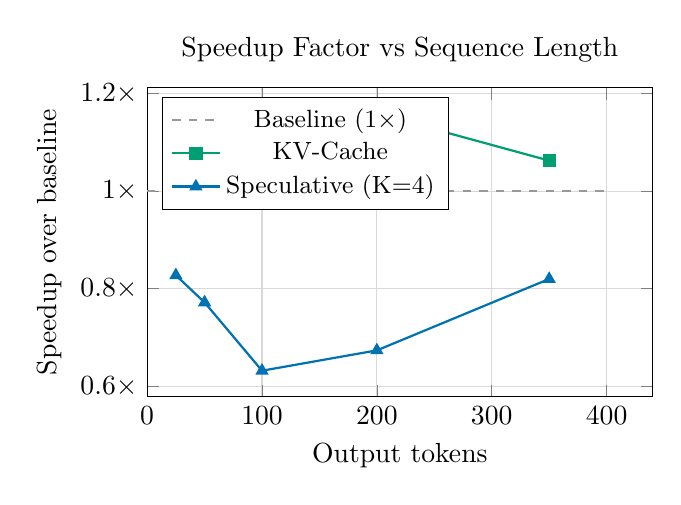
\begin{tikzpicture}
\begin{axis}[
  width=8cm, height=5.5cm,
  xlabel={Output tokens},
  ylabel={Speedup over baseline},
  title={Speedup Factor vs Sequence Length},
  legend pos=north west,
  legend style={font=\small},
  grid=major, grid style={gray!30},
  xmin=0,
  yticklabel={\pgfmathprintnumber[fixed,precision=1]{\tick}$\times$},
]
\addplot[dashed, grey, thick] coordinates {(0,1) (400,1)};
\addlegendentry{Baseline (1$\times$)}
\addplot[color=teal, mark=square*, thick] coordinates {(25,1.0649) (50,1.0347) (100,1.0365) (200,1.1590) (350,1.0626)};
\addlegendentry{KV-Cache}
\addplot[color=blue, mark=triangle*, thick] coordinates {(25,0.8275) (50,0.7719) (100,0.6319) (200,0.6736) (350,0.8200)};
\addlegendentry{Speculative (K=4)}
\end{axis}
\end{tikzpicture}
\end{document}
